\chapter[EAS Selection Efficiency with Increased NSB]{\centering EAS Selection Efficiency \\ with Increased NSB \\}\label{Ch:SelectEff}


%Selection Efficiency of EAS under increased NSB
%\begin{itemize}
%\item Smearing real data with extra noise
%\item Simulating EAS with an increased NSB
%\item Talk about differences in smearing and simulating EAS (different triggering conditions)
%\item Energy and Xmas resolution and bias
%\item Rp bias
%\item differences in track length
%\end{itemize}

\section{Motivation}

The FD shifts are typically organised for night with the illuminated fraction of the moon less then 70\% and can be operated longer than 3 hours of moon below the horizon. The Fd telescope shutters are then opened when the sun is below -18\textdegree of the horizon (astronomical twilight), the average variance of the camera PMTs less then 100 ADC$^2$ and individual PMTs less then 2000 ADC$^2$. Two calculations where done by the collaboration to estimate the theoretical up time of the FD's. Before 2012 the theoretical calculations looked like:

\begin{table}[h]
\centering
\begin{tabular}{c c}
Theoretical up time & 22\% \\
Loss due to shor nights ($<$ 3 hrs) & -2\% \\
Loss due to bad weather or fails & -5\% \\ \hline \hline
Total measurement time & 15\% 
\end{tabular}
\end{table}

For context the measured ADC$^2$ for typically observed Night Sky Background (NSB) with no moon, quarter moon and full moon/twilight is:
\begin{table}[h]
\centering
\begin{tabular}{c c c}
\hline\hline
Condition & $\sigma^2$ [ADC$^2$] & I$_{\mathrm{a}}$ [$\mu$A] \\ \hline\hline
no moon & 25 & 0.5 \\
quarter moon & 250 & 5 \\
full moon/twilight & 2500 & 50 \\ \hline\hline
\end{tabular}
\end{table}

These values are measured under the standard operation of the FD's. Further within this thesis I will investigate lower the gain on the PMTs to reduce the variance and current that their under. A lower current when observing under moonlight would help make sure that the PMT lifespans are not changed by the increased in NSB.

The signal that the FD's observe is AC coupled, which means the mean signal of the NSB is zero. Instead the variance around zero is calculated andis directly proportional to the fluctuations in the NSB. The average value of the NSB measured by POA at Malargue is:
\begin{equation}
\sigma^2 \sim 25 \ \mathrm{ADC}^2
\end{equation}
The variance in ADC$^2$ can be converted into photons seen at the aperture by using:
\begin{eqnarray}
\sigma^2_{pe} &=& [\sigma^2_{\mathrm{ADC}}]^{\mathrm{sky}} \ / \ \mathrm{A}^2_{\mathrm{G}} \label{eq:simgaPE} \\
\mathrm{n}_{\mathrm{ph}} &=& \frac{\sigma^2_{pe}}{(1 + \mathrm{V}_{\mathrm{G}})} \label{eq:numPhoton}
\end{eqnarray}
where $\sigma_{pe}$ is the standard deviation of the photo-electron count, n$_{\mathrm{ph}}$ is the photon count and A$_{\mathrm{G}}$ is equal to:
\begin{equation}\label{eq:abs_gain}
\mathrm{A}_{\mathrm{G}} = \frac{1}{\mathrm{C}_{\mathrm{FD}}.\mathrm{f}.\mathrm{Q}}
\end{equation}
where
\begin{itemize}
\item[] A$_{\mathrm{G}}$ is the absolute gain (ADC/photo-electron)
\item[] $\mathrm{C}_{\mathrm{FD}}$ is the FD pixel calibration constant.
\item[] Q is the Quantum efficiency of the PMT.
\item[] f is the efficiency if the telescope optics.
\end{itemize}

/*------ \textbf{Find reference to number below} ------*/

Assuming typical measured values for C$_{\mathrm{FD}}$, Q and f shown in:

\begin{center}
\begin{tabular}{|c|c|}
\hline
C$_{\mathrm{FD}}$ & 4.5 photons/ADC \\
\hline
Q & 0.29 \\
\hline
f & 0.465 \\
\hline
\end{tabular}
\end{center}

Therefore can now calculate A$_{\mathrm{G}}$ from Eq. \ref{eq:abs_gain} and using 



- Need graph of expected variance in ADC$^2$ for the moon above the horizon for different phases.

- Want to increase the duty cycle of FD by measuring EAS under moonlight. Most likely observe under quarter to half moon. This will increased the NSB upto a factor of 10.

- The aim of increasing the duty cycle of FD is too measure more EAS at the highest energy band ($> 10^{19.5}$ eV).

- Need more statistics at highest energy band to complement SD measurements.


\section{Selection Efficiency}

I investigated a couple of method evaluating increasing the NSB by different factors. The main increase of NSB will be from half moon which equates to an increase in NSB by a factor of 10. The two methods involved simulating increased NSB on measured data and with simulating. The measured data had increased noise introduced across the entire signal trace and I have labelled as the smearing method.

Selection Efficiency for the two methods are calculated via:
\begin{equation}
\mathrm{Efficiency} = \mathrm{N}_{\mathrm{Selected}} / \mathrm{N}_{\mathrm{total}}
\end{equation}
where for the Smearing method N$_{\mathrm{total}}$ is the total number of measured EAS events at standard NSB levels and N$_{\mathrm{Selected}}$ is the number of events after being reconstructed and passing the quality cuts with the increased NSB. For the simulations, N$_{\mathrm{total}}$ is the total number of simulated events before \textbf{need to check whether its the number of simulations before triggering or number of triggered events at standard NSB}.

Smearing method involves taking fluorescence telescope EAS data that have been reconstructed and passed all of the quality cuts and adding addition random variance in ADC$^2$ equivalent to an increased NSB from moonlight. The EAS data is then reconstructed and passed through the same quality cuts. This a repartition of a similar method that M. Unger had preformed in \textbf{2012}. \textbf{Also need to refer to the study done by Brue and Andrew Smith around 1999}. This was done so a deeper analysis could be preformed to understand the underlying mechanics.

The simulations were done using the simulation modules for the FD's within the OffLine analysis programs. The EAS profiles were generated within CONEX and the original showers were generated through CORSIKA. The NSB was added to the EAS profiles before the FD are triggered. A hybrid trigger is used to involve the SD but the SD is simulated in asimple way just to get a simulated core position.

The smearing method was used as a proof of concept to show that EAS showers could still be reconstructed with the increased NSB. The limitation was that EAS were used that already triggered the FD's normally. The full simulation using CONEX showers was used to full test trigger conditions through to reconstruction. The simulations are not an 100\% accurate representation of the POA array so that will introduce some differences too.


\begin{figure}[!hp]
\centering
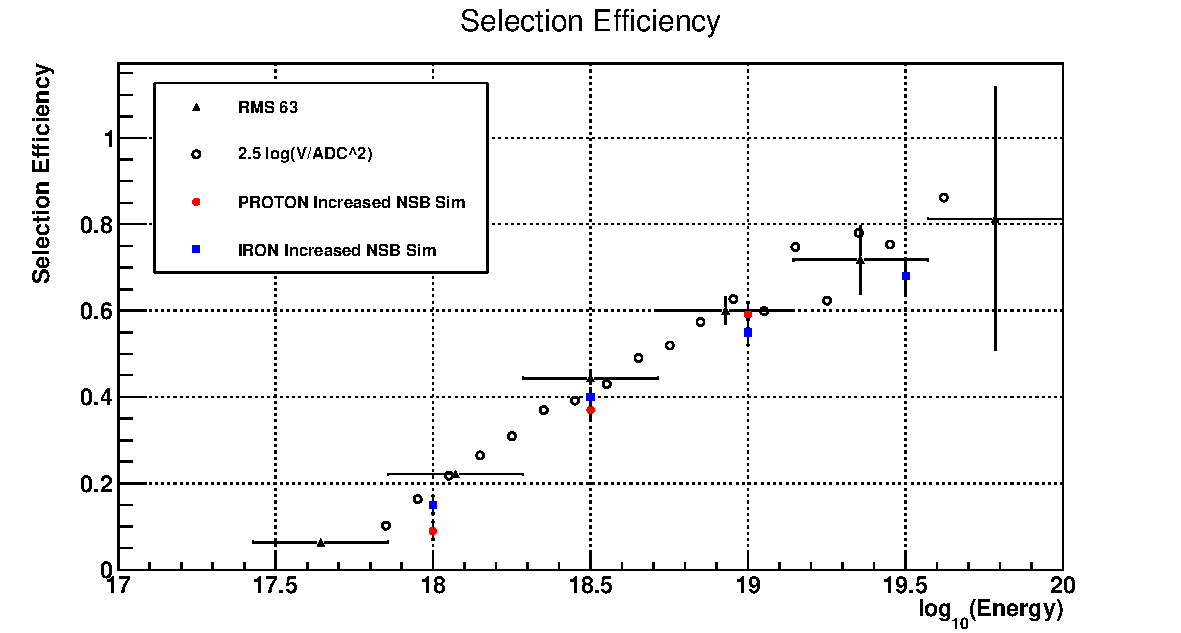
\includegraphics[width=\textwidth]{chapters/graphs/SelectionEff/SelectionEff_errorbars_10timesNSB.pdf}
\caption{Selection Efficiency plot containing data from both the Smearing method and simulated showers. These results are compared to the work done by M. Unger.}
\end{figure}

\section{Resolution and Bias}

To further evaluate the effects of increasing the NSB on the quality of the reconstructed EAS data, I look at the resolution and bias of both the reconstructed energy and reconstructed Xmax. A quick reminder that Xmax is the measurement of the brightest part of the shower relating to the maximum number of particles produced. For the smearing method the energy and Xmax bias is comparing to the measured data taken at standard NSB levels to the reconstructed with the increased NSB levels. For the simulations the energy and Xmax bias can be calculated using the true energy and Xmax values used to generate each EAS profile.

The trend of the energy resolution for both methods is that as the energy of the EAS event increases the bias decreases. This was expected as the energy of the shower increases the brighter and longer the track that is observed. A brighter and longer track allows for a better reconstruction.

- Need to find out what's a good bias value for energy and Xmax.

the energy and Xamx bias is calcualted via:
\begin{eqnarray}
\Delta \mathrm{E} &=& \frac{\mathrm{E}_{\mathrm{recon}} - \mathrm{E}_{\mathrm{true}}}{\mathrm{E}_{\mathrm{true}}} \\ 
\Delta \mathrm{E} &=& \frac{\mathrm{E}_{\mathrm{IncreasedNSB}} - \mathrm{E}_{\mathrm{StandardNSB}}}{\mathrm{E}_{\mathrm{StandardNSB}}} \\
\Delta \mathrm{Xmax} &=& \mathrm{Xmax}_{\mathrm{recon}} - \mathrm{Xmax}_{\mathrm{true}} \\
\Delta \mathrm{Xmax} &=& \mathrm{Xmax}_{\mathrm{IncreasedNSB}} - \mathrm{Xmax}_{\mathrm{StandardNSB}}
\end{eqnarray}

The energy and Xmax resolution is calculated via:
\begin{eqnarray}
\sigma_{\mathrm{res}} &=& \left( \frac{1}{\mathrm{N}} \sum \frac{1}{\sigma^2_i} \right)^{1/2}
\end{eqnarray}


\begin{figure}
\centering
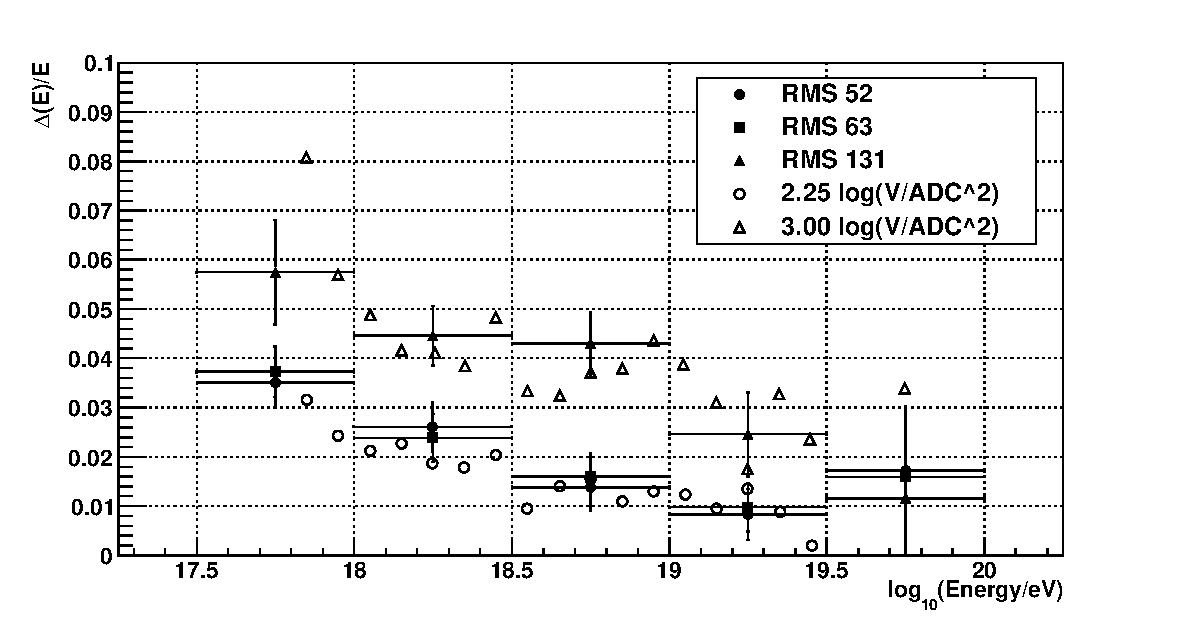
\includegraphics[width=\textwidth]{chapters/graphs/SelectionEff/Smearing_RealData_EnergyBias.pdf}
\caption{Energy Bias using Smearing Method.}
\vspace{3mm}
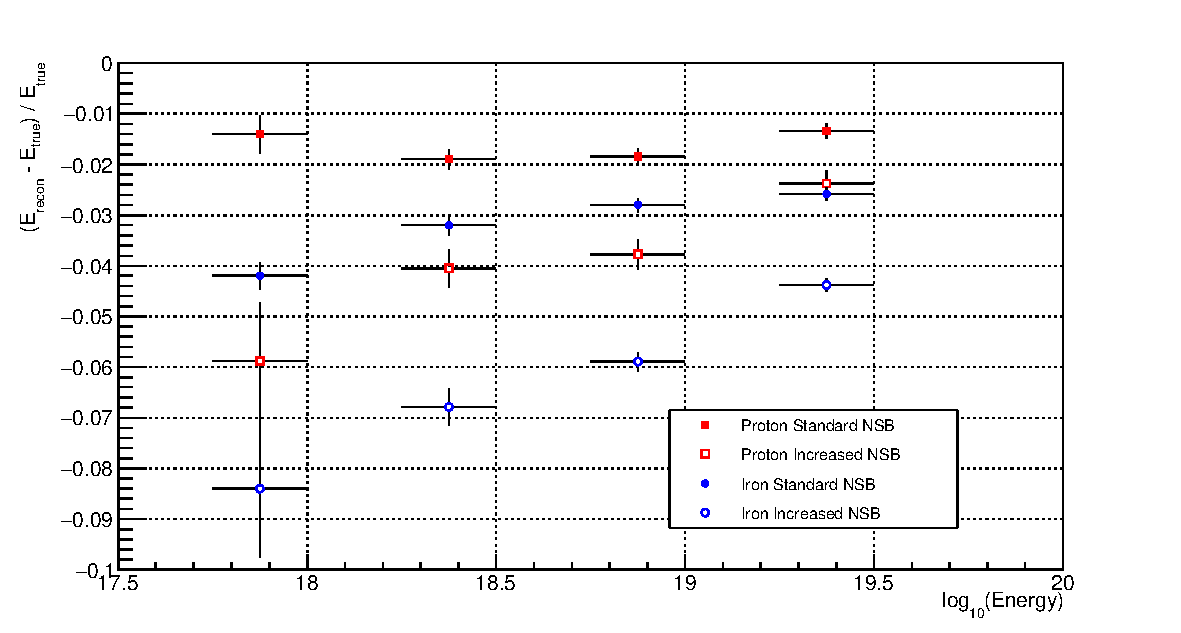
\includegraphics[width=\textwidth]{chapters/graphs/SelectionEff/Simulation_ProtonIron_EnergyBias.pdf}
\caption{Energy Bias using simulated data.}
\end{figure}

\begin{figure}
\centering
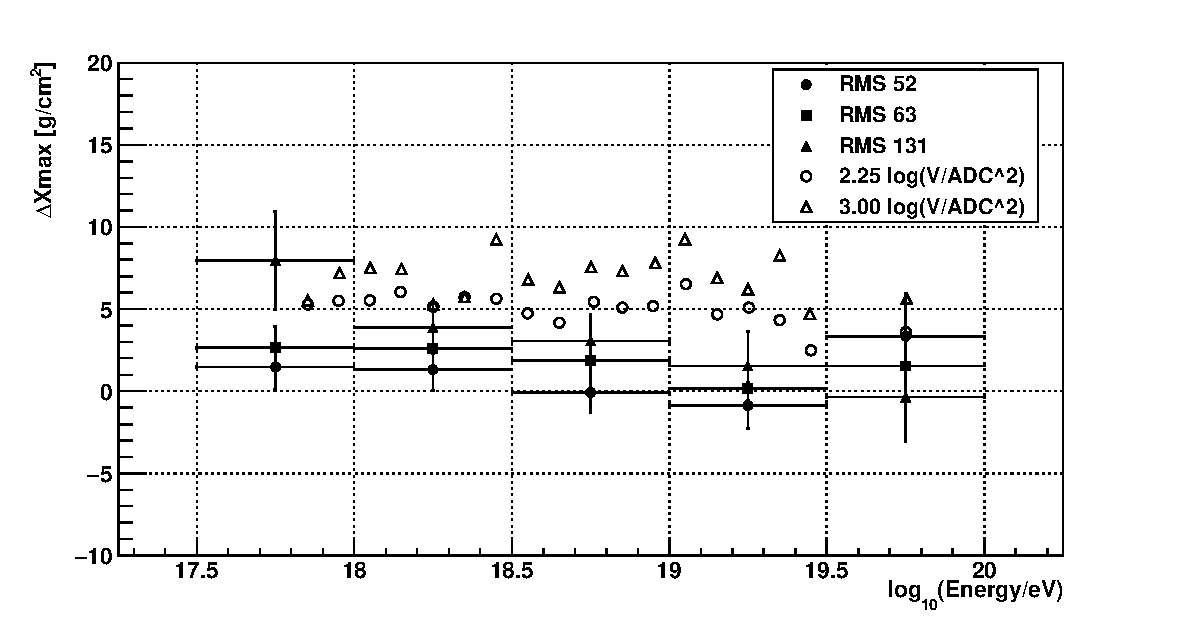
\includegraphics[width=\textwidth]{chapters/graphs/SelectionEff/Smearing_RealData_XmaxBias.pdf}
\caption{Xmax Bias using Smearing Method.}
\vspace{3mm}
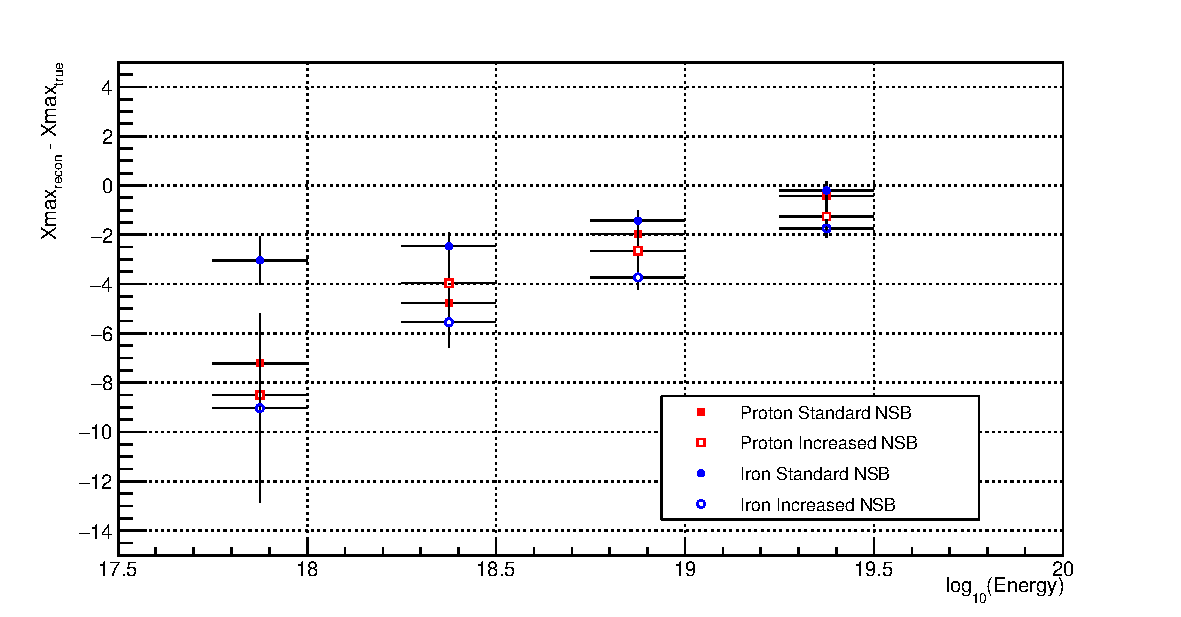
\includegraphics[width=\textwidth]{chapters/graphs/SelectionEff/Simulation_ProtonIron_XmaxBias.pdf}
\caption{Xmax Bias using simulated data.}
\end{figure}

\begin{figure}
\centering
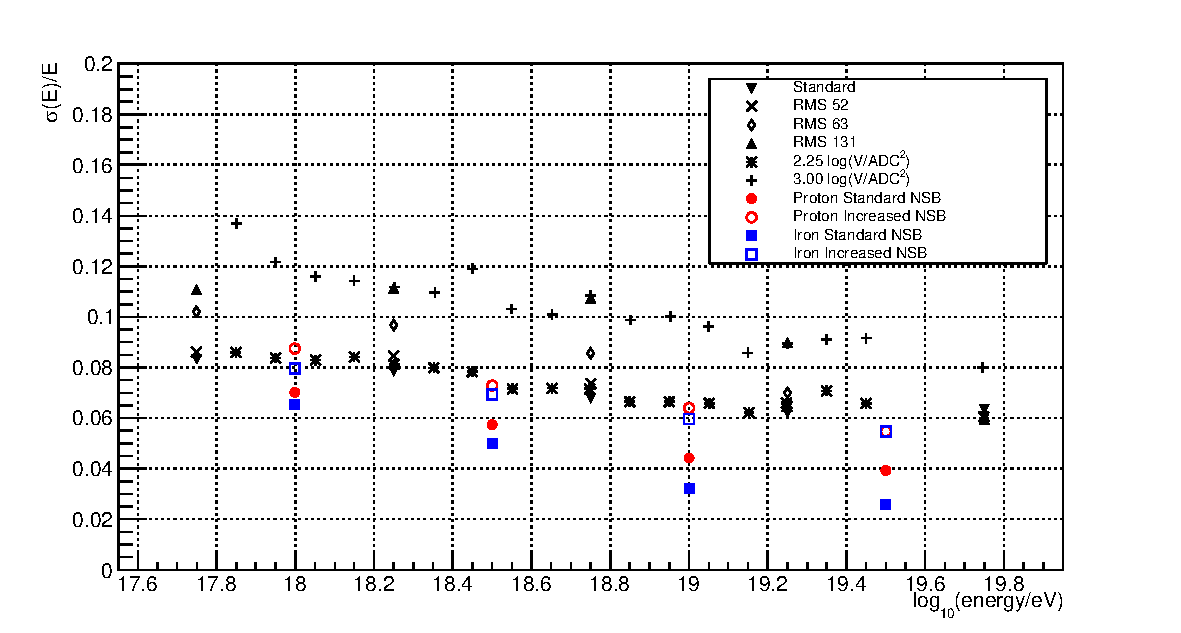
\includegraphics[width=\textwidth]{chapters/graphs/SelectionEff/Combined_EnergyRes_All.pdf}
\caption{Energy Resolution using both Smearing Method data and simulated showers.}
\vspace{3mm}
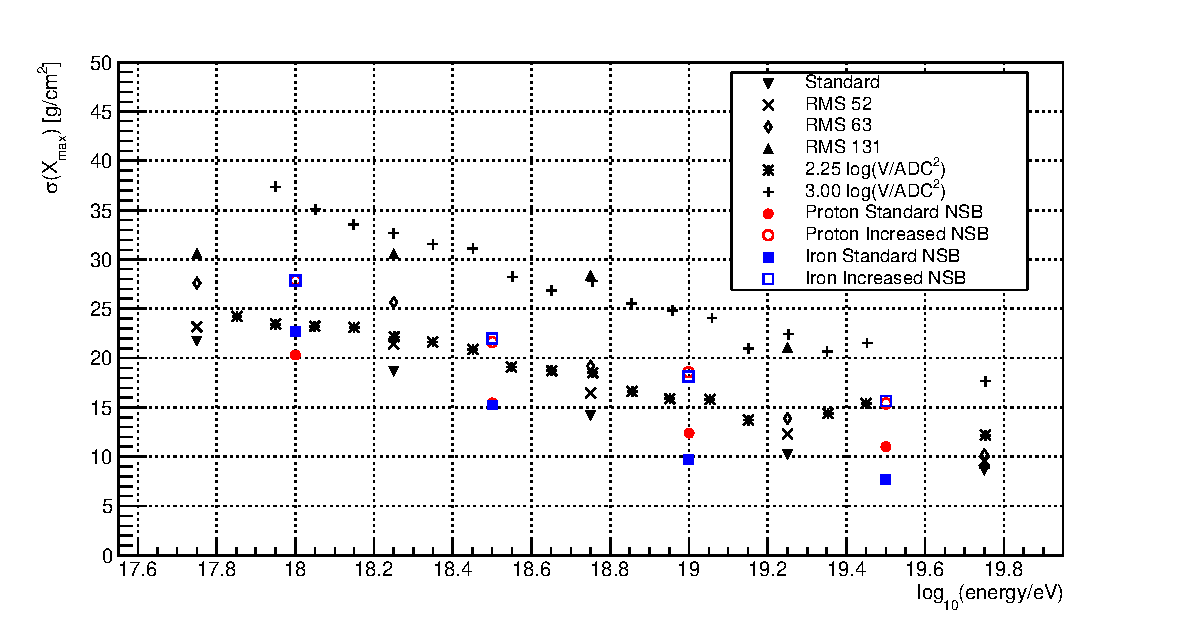
\includegraphics[width=\textwidth]{chapters/graphs/SelectionEff/Combined_XmaxRes_All.pdf}
\caption{Xmax Resolution using both Smearing Method data and simulated showers.}
\end{figure}

\subsection{Comparing Simulated Data to Real Data}

\textbf{Think about where to locate this section.}

Comparing the simulated data with real data. Checking to make sure that the simulation data is a good representation of reality. Looking at the Xmax distribution there is no need for a direction comparison as I only simulated proton and iron primaries and was not concern with have a particular mixtures. The other parameter I checked was the zenith angle distribution, distance to Xmax and distance to the shower axis (R$_{\mathrm{P}}$). The simulated profiles have similar shapes when both histograms are normalised to area of 1. For zenith angle distribution I simulated the EAS events upto a zenith angle of 60\textdegree so that the reason for the cut-off in the simulated data.

\begin{figure}
\centering
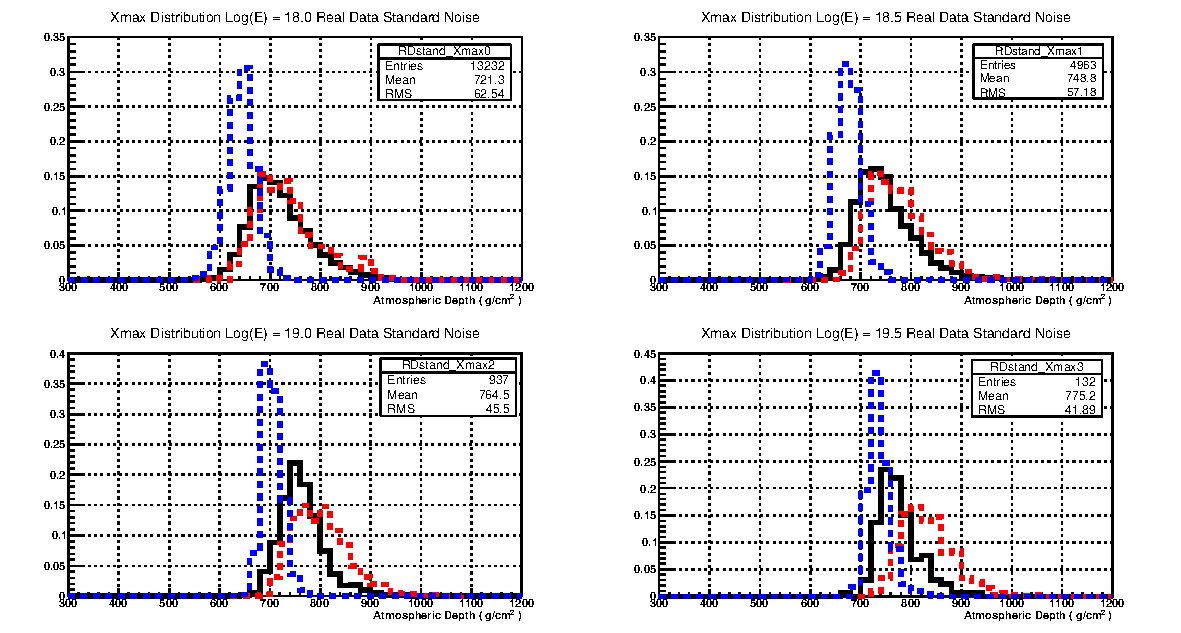
\includegraphics[width=\textwidth]{chapters/graphs/SelectionEff/RealDataAndSim_XmaxDistComp.pdf}
\caption{Distribution of Xmax with Real Data and simulation of proton and iron showers.}
\vspace{3mm}
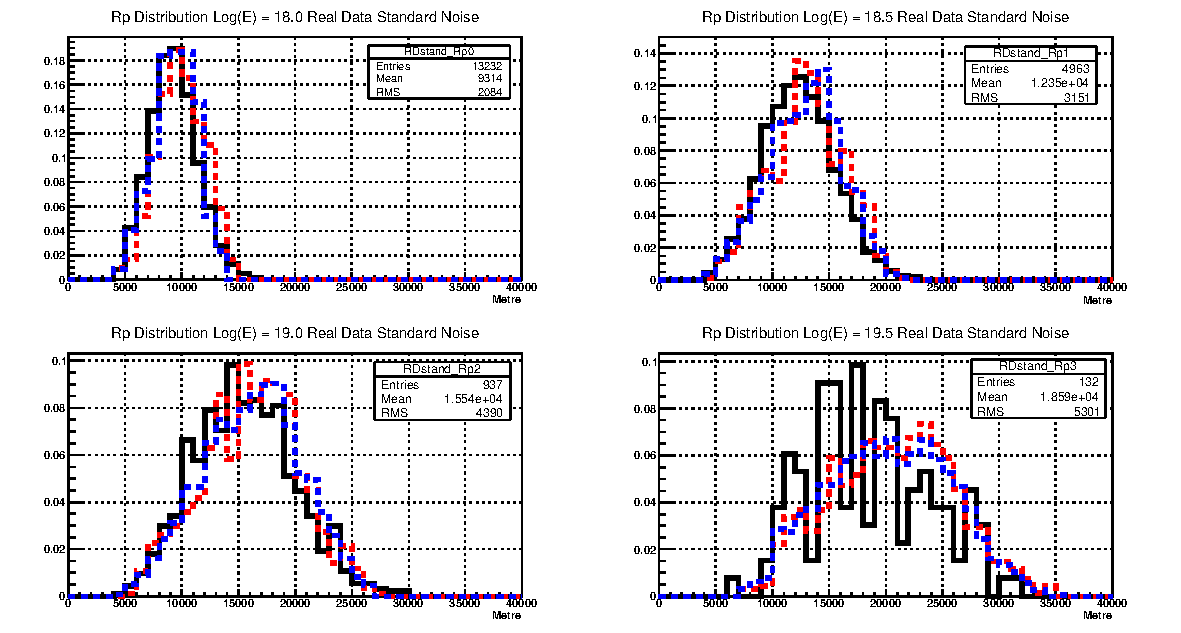
\includegraphics[width=\textwidth]{chapters/graphs/SelectionEff/RealDataAndSim_RpDistComp.pdf}
\caption{Distribution of Rp with Real Data and simulation of proton and iron showers.}
\end{figure}

\begin{figure}
\centering
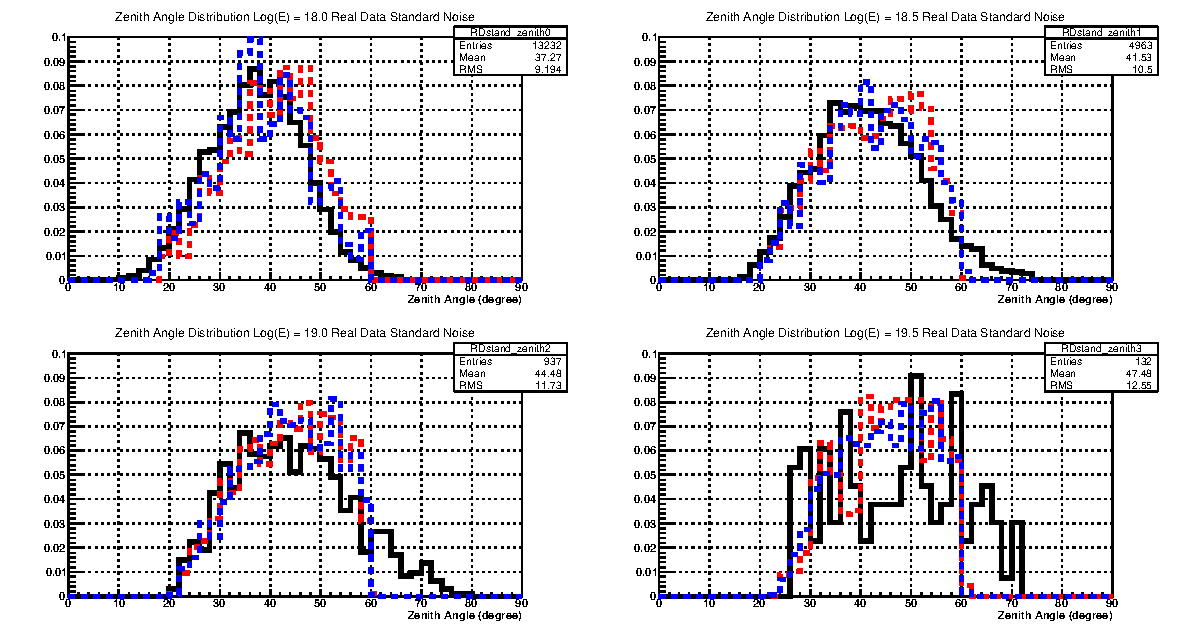
\includegraphics[width=\textwidth]{chapters/graphs/SelectionEff/RealDataAndSim_ZenithDistComp.pdf}
\caption{Distribution of Zenith angle with Real Data and simulation of proton and iron showers.}
\vspace{3mm}
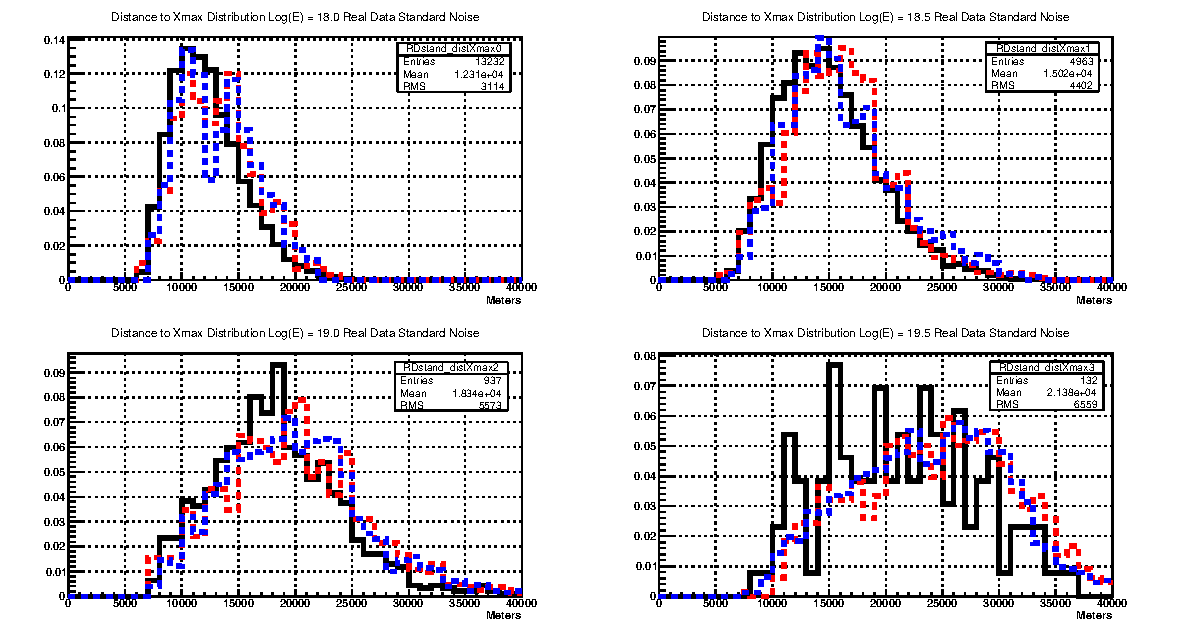
\includegraphics[width=\textwidth]{chapters/graphs/SelectionEff/RealDataAndSim_DistToXmaxDistComp.pdf}
\caption{Distribution of Distance to Xmax with Real Data and simulation of proton and iron showers.}
\end{figure}

\section{EAS Track Length in the FD's}

One other parameter that was investigate was the shower track length observed by the FD's. It was expected that as the NSB increased the average observed shower track length would decrease. 

\begin{figure}
\centering
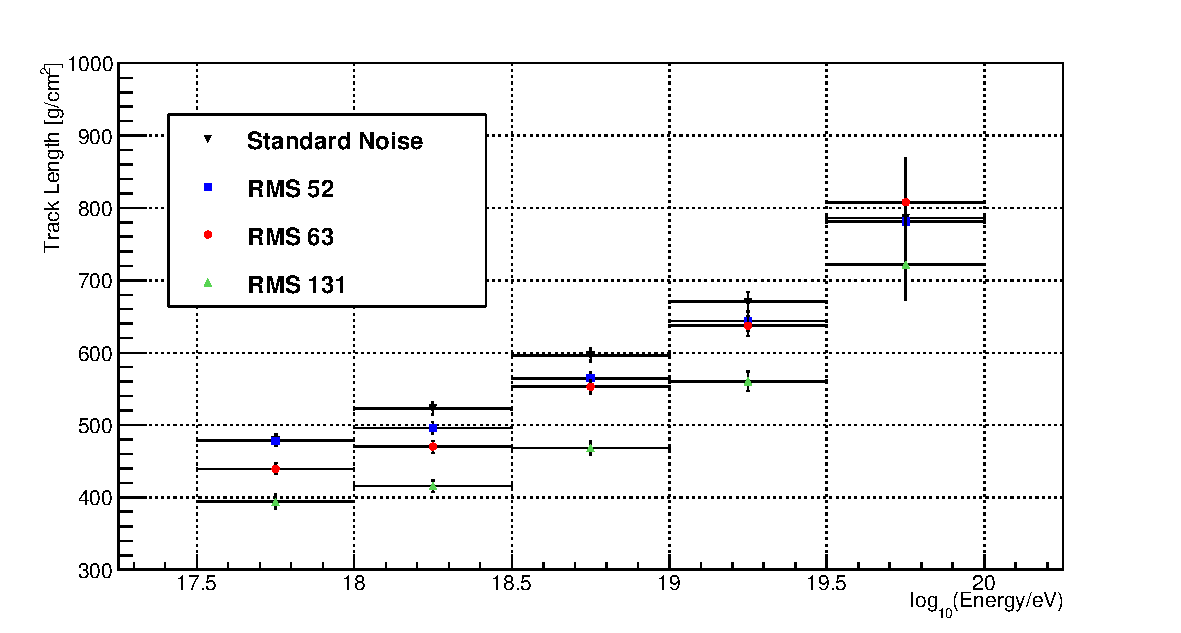
\includegraphics[width=\textwidth]{chapters/graphs/SelectionEff/Smearing_TrackLength_DiffNSBlevels.pdf}
\caption{Track length using Smearing method.}
\vspace{3mm}
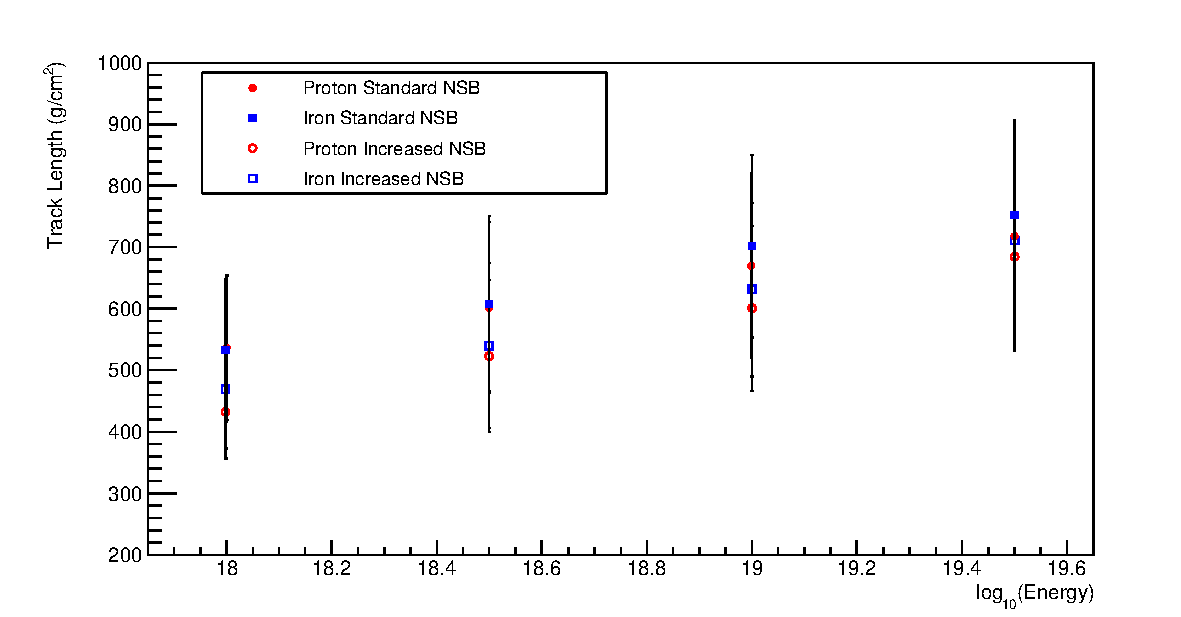
\includegraphics[width=\textwidth]{chapters/graphs/SelectionEff/Simulation_TrackLength_Comb_StandANdIncreasedNSB.pdf}
\caption{Track length using simulation of proton and iron CONEX showers.}
\end{figure}
